% ----------
% A LaTeX template for course project reports
% 
% This template is modified from "Tech Report ala MIT AI Lab (1981)"
% 
% ----------
\documentclass[12pt, letterpaper, twoside]{article}
\usepackage{geometry}
\usepackage[utf8]{inputenc}
\usepackage[english]{babel}
\usepackage[runin]{abstract}
\usepackage{titling}
\usepackage{booktabs}
\usepackage{fancyhdr}
\usepackage{helvet}
\usepackage{csquotes}
\usepackage{graphicx}
\usepackage{blindtext}
\usepackage{parskip}
\usepackage{etoolbox}
\usepackage{hyperref}

\documentclass{article}
\usepackage{float} % For H float option
%\input{preamble.tex}

% ----------
% Variables
% ----------

\title{\textbf{ICSHelper}} % Full title of your tech report
%\runningtitle{On Image Matting} % Short title
\author{Ahila, Pawan, Shutong Wu, Yi-Leng Chen \and [rameshra,kumarp40,wu867,cheny997]@mcmaster.ca} % Full list of authors
%\runningauthor{Student Name 3 et al.} % Short list of authors


% ----------
% actual document
% ----------
\begin{document}
\maketitle

\begin{abstract}
    An ICS (iCalendar) file is a universal calendar format utilized by mainstream email and various calendar apps such as Microsoft Outlook, Google Calendar, and Apple Calendar. Importing an ICS file into calendar apps allows for the addition of new schedules comprising one or more events. Currently, the process of manipulating ICS files involves editing schedules within calendar apps and then exporting them. To address this time-consuming task, we propose ICS Helper, a Domain-specific Language (DSL) designed for handling ICS files. It's a text based tool kit that allow users to generate schedules outside of calendar applications, and provides integration possibility as an Eclipse plugin. With its user-friendly syntax, ICS Helper enables users to manage their schedules more effectively. 
\end{abstract}

\vspace{2.5cm}

% Uncomment the following to add thanks.
% {\footnotesize
%     \noindent
%     Special thanks to \textbf{Person 1} and \textbf{Affiliation A} for financial support for this project.
% }

\thispagestyle{firstpage}

\pagebreak
% ----------
% End of first page
% ----------

\newgeometry{} % Redefine geometries (normal margins)

\section{Introduction}
\label{sec:intro}
An ICS file is a calendar file saved in a universal calendar format used by mainstream email and calendar apps, including Microsoft Outlook, Google Calendar, and Apple Calendar. 

By importing ICS file into calendar apps, a new schedule(composed of one or more events) can be added. People can subscribe to schedules by url. 

Right now the only way to manipulate ICS files (other than writing the protocol by hand) is to edit schedules inside calendar apps / helpers, and then export, which hinders:

    \begin{itemize}
        \item easy creation of schedules outside the app environment
        \item mass operation (e.g. delay 100 events by an hour) 
        \item programmable access (e.g. work flow automation)
        \item granular control(e.g. split and merge of events across schedules)
    \end{itemize}


To tackle this, we propose the idea of `ICS Helper`, which is a DSL dealing with ICS files. It offers:
    \begin{itemize}
        \item human-friendly syntax for ICS creation (write in plain text & compile to ICS)
        \item model validation (e.g. time conflict, missing fields)
        \item integration options with other tools as a plugin
    \end{itemize}

While it doesn't solve all the problems mentioned, it provides a good starting point for further development.

The DSL will be implemented using \texttt{Xtext}, and the project will be shipped as a plugin for Eclipse.
\newpage
\section{Metamodel Definition and Analysis}

The metamodel defined using Emfatic/Ecore serves as the foundation for the ICS Helper DSL. Below is the metamodel along with an analysis of its components, assumptions, and alternative design considerations.

\subsection{Metamodel Overview}

The metamodel defines the structure and relationships of entities within the ICS Helper DSL. It comprises five main classes: \texttt{Schedule}, \texttt{Location}, \texttt{Organizer}, \texttt{Invitee}, and \texttt{Event}. These classes encapsulate various aspects of scheduling and event management.

\begin{itemize}
    \item \textbf{Schedule}: Represents a schedule containing multiple events. It includes attributes for name and description, along with associations with events and the schedule owner.
    
    \item \textbf{Location}: Represents the physical or virtual location of an event. It contains an attribute for the address.
    
    \item \textbf{Organizer}: Represents the organizer of a schedule or event. It includes attributes for name and email, as well as an association with a location.
    
    \item \textbf{Invitee}: Represents an individual invited to an event. It includes attributes for name and email.
    
    \item \textbf{Event}: Represents a specific event within a schedule. It includes attributes for title, description, start date, end date, and recurrence. It also has associations with attendees, the parent schedule, and the event location.
\end{itemize}

\subsection{Assumptions}

The metamodel assumes certain characteristics of schedules, events, organizers, and invitees:

\begin{itemize}
    \item Events can have multiple attendees.
    \item Events are part of a schedule.
    \item Organizers and invitees have associated email addresses.
    \item Each event has a single location.
\end{itemize}

\subsection{Alternative Design Considerations}

While the current metamodel provides a solid foundation, alternative design considerations could enhance its flexibility and completeness:

\begin{itemize}
    \item Event Recurrence: Consider defining a separate class for recurring events to handle more complex recurrence patterns.
    \item Polymorphism for Locations: Instead of a single \texttt{Location} class, explore the possibility of different location types represented by subclasses.
    \item Event Timezone: Incorporate timezone information for events, especially when dealing with events across different time zones.
\end{itemize}

\subsection{Class Diagram}

The following class diagram visually represents the structure and relationships defined in the metamodel:

\begin{figure}[H]
    \centering
    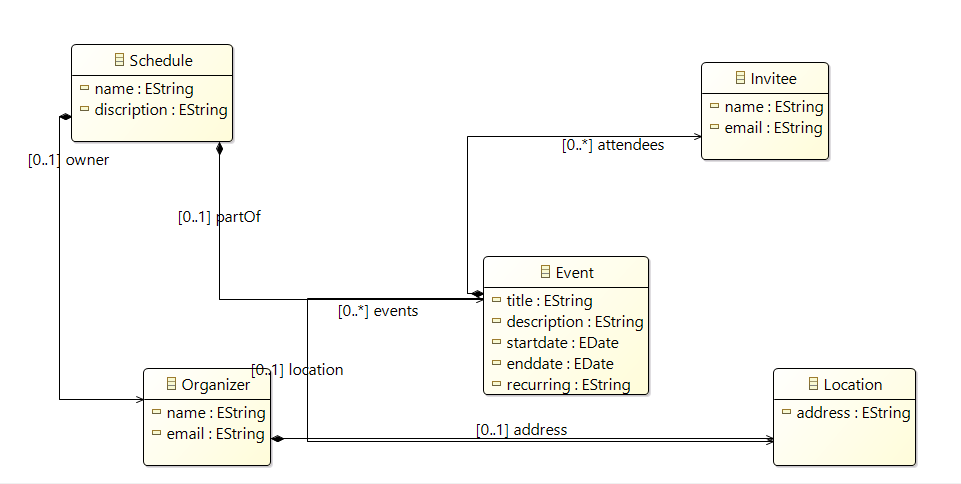
\includegraphics[width=0.7\textwidth]{class.png}
    \caption{Class Diagram of the ICS Helper DSL Metamodel}
    \label{fig:class-diagram}
\end{figure}

The diagram illustrates the associations between the main entities, providing a visual reference for the metamodel.

This metamodel analysis and class diagram form the basis for the subsequent development and implementation of the ICS Helper DSL.


\newpage
\section{Defining and Implementing Syntax}
We choose \texttt{Xtext} to implement the syntax and generate editor accordingly for the below reasons:

\begin{itemize}
    \item \texttt{Xtext}, as a text-based tool, provide flexible syntax control.
    \item Consider the use case of our dsl, usability in a text-based environment is a must.
    \item Better integration with other platforms and tools.
\end{itemize}

\subsection{Syntax}
Aiming to be user-friendly and intuitive, the syntax of ICS Helper DSL is designed to be concise and natural-language-like. 
The following sections outline the syntax elements and examples of the DSL.
\subsubsection{Basic Syntax}
\begin{verbatim}
    'create' 'schedule' UNIQUE_NAME '{'
        one or more Event
    '}'
\end{verbatim}

Where \texttt{Event} is defined as follows:

\begin{verbatim}
    'event' UNIQUE_NAME
    'start' YYYY-MM-DD HH:MM:SS
    'end' YYYY-MM-DD HH:MM:SS
    (OPTIONAL FIELDS)
\end{verbatim}
OPTIONAL FIELDS include: \texttt{location}, \texttt{description}, \texttt{organizer}, \texttt{invitees}, \texttt{recurrence rule}, \texttt{reminder rule}, \texttt{link}. 
Please refer to \href{https://github.com/Gudauu/ICS-Helper}{our documentation} for more details.

\subsubsection{example}
\begin{figure}[H]
    \centering
    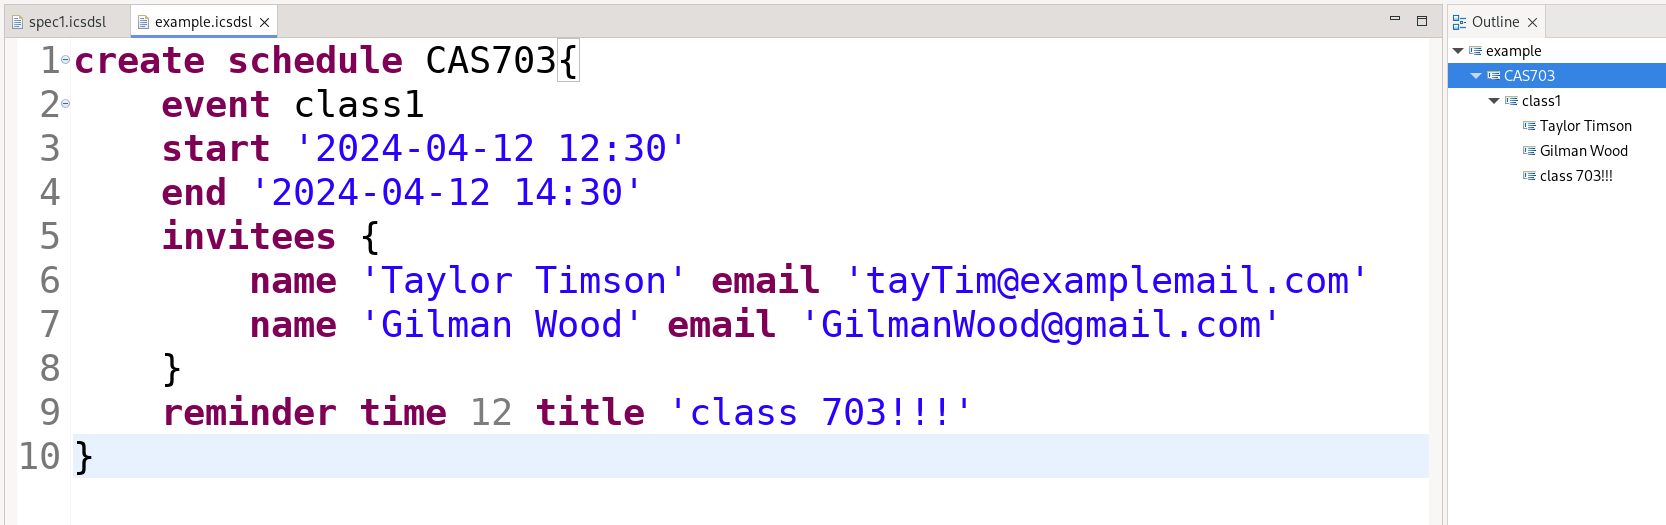
\includegraphics[width=0.7\textwidth]{editor_example.png}
    \caption{Example Editor Screenshot}
    \label{fig:class-diagram}
\end{figure}

\begin{verbatim}
    create schedule CAS703{
        event class1 
        start '2024-04-12 12:30'
        end '2024-04-12 14:30'
        invitees {
            name 'Taylor Timson' email 'tayTim@examplemail.com'
            name 'Gilman Wood' email 'GilmanWood@gmail.com'
        }
        reminder time 15 title 'go to class 703!!!'
    }
\end{verbatim}

\subsection{Discussion}
Our syntax design using \texttt{Xtext} comes with the following advantages:
\begin{itemize}
    \item Friendly syntax that is easy to understand and use.
    \item Editor that provides syntax highlighting, auto-completion, and error checking.
    \item Portability and integration with other tools (as our project is shipped as a plugin). 
\end{itemize}
At the same time, it comes with the following limitations:
\begin{itemize}
    \item Dependence on the Eclipse environment.
    \item Grammar limitations: like the need to follow the time format exactly, which hinders easy-usage.
    \item Higher learning curve compared to graphical editors.
\end{itemize}


\newpage
\section{Validation constraints implementation}
To better check the correctness, this project separate the validation into two parts.

\subsection{Epsilon Validation Language (EVL)}
To validate aspects of the model that couldn't be expressed in the metamodel itself, we use EVL (Epsilon Validation Language) constraints to achieve our goal. Below are the constraints we have set up:
\begin{enumerate}
    \item \textbf{Not null or empty constraints:}
    \begin{itemize}
        \item Schedule Class: The name of the schedule must not be null or empty.
        \item Organizer Class: The name of the organizers must not be null or empty.
        \item Invitee Class: The name of the invitees must not be null or empty.
        \item Event Class: The name of the event must not be null or empty.
    \end{itemize}
    \item \textbf{Unique constraints:}
    \begin{itemize}
        \item Organizer Class: The email address of the organizers must not be duplicated.
        \item Invitee Class: The email address of invitees must not be duplicated.
    \end{itemize}
    \item \textbf{Time constraints:}
    \begin{itemize}
        \item Event Class: The event's start time must not be later than its end time.
    \end{itemize}
\end{enumerate}
\subsection{Xtext editor vaildation}
To enhance compatibility with the Xtext editor, we use Java for runtime validation of events. Below are the constraints we have established:
\begin{enumerate}
    \item \textbf{Time constraints:}
    \begin{itemize}
        \item The event's start time cannot be later than its end time.
        \item The event's reminder time must not be less than 0 minutes.
    \end{itemize}

    \item \textbf{Email constraints:}
    \begin{itemize}
        \item The emails of the organizer and invitees must follow the general email format.
        \item The emails of the organizer and invitees cannot be null or empty.
        \item The emails of the organizer and invitees must be unique and not repeated.
    \end{itemize}

    \item \textbf{Additional constraint:}
    \begin{itemize}
        \item The event link should resemble a URL, i.e., it should contain "://" to indicate it is a URL.
    \end{itemize}
\end{enumerate}

The figure above displays some outcomes of running the validation code, checking the start and end times of the event, as well as verifying the event link.
\begin{figure}
    \centering
    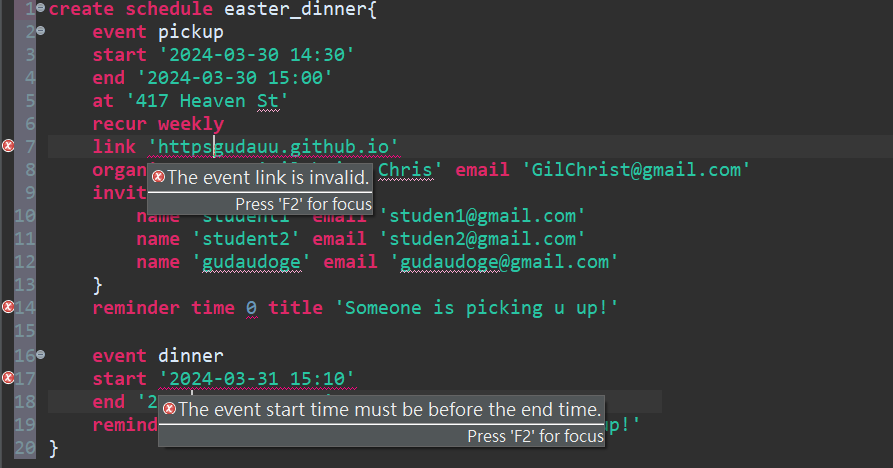
\includegraphics[width=1\linewidth]{xtext validation.png}
    \caption{Xtext validation example}
    \label{fig:enter-label}
\end{figure}
\newpage
\section{Model management operation implementation}
Since the goal of our DSL is to generate ICS files, we implemented the model-to-text transformation operation. 

The operation takes an .icsdsl file (our DSL file) as input and generates a corresponding .ics file as output, which can be further imported into calendar applications.

\subsection{Implementation}

The operation is implemented using \texttt{Xtend}, a statically-typed programming language that compiles to Java. 
\texttt{Xtend} is used in accordance with \texttt{Xtext} to provide seamless code translation and execution. 

The operation reads the .icsdsl file, then for each \texttt{CreateCommand}, read the values assigned to each mandatory and optional field, and translate them into the corresponding .ics format.

For instance, the below \texttt{Xtend} code translates the \texttt{organizer} field.
\begin{verbatim}
    if (event.organizer !== null) {
        icsContent.append("ORGANIZER;CN=" + 
        event.organizer.name + ":mailto:" 
        + event.organizer.email + "\n")
    }
\end{verbatim}

\subsection{Example}
The example ICS snippet shown in 3.1.2 will be transformed into CAS703.ics with content below:
\begin{verbatim}
    BEGIN:VCALENDAR
    VERSION:2.0
    PRODID:-//hacksw/handcal//NONSGML v1.0//EN
    BEGIN:VEVENT
    SUMMARY:class1
    DTSTART:20240412T123000Z
    DTEND:20240412T143000Z
    ATTENDEE;CN="Taylor Timson":MAILTO:tayTim@examplemail.com
    ATTENDEE;CN="Gilman Wood":MAILTO:GilmanWood@gmail.com
    RRULE:FREQ=DAILY
    BEGIN:VALARM
    TRIGGER:-PT12M
    ACTION:DISPLAY
    DESCRIPTION:class 703!!!
    END:VALARM
    END:VEVENT
    END:VCALENDAR
\end{verbatim}

\subsection{Limitations and future work}
One limitation in the model transformation (and subsequently affecting the syntax definition) would be the strict syntax requirements.  

For instance, the time should be specified in exactly 'YYYY-MM-DD HH:MM:SS' format, which might be inconvenient.

This can be easily (but time-consumingly) solved by supporting more time formats in the \texttt{Xtend} transformation code.





\newpage

\section{References}

\end{document}

% ----------